%! Author = sriadityavedantam
%! Date = 4/7/26

\section{Zariski Topology}

\begin{lemma*}{
    An affine variety is a Zariski closed subset together with its ring of regular functions.
}
\end{lemma*}

\begin{definition}[Regular Function]
    Let $Z\subseteq \aa^n$.
    A regular function on $Z$ is a map $f|_Z : Z\to \kk$ induced by a polynomial $f\in \kk[x_1,\ldots,x_n]$.

    There is a quotient map
    \[
        I(Z)\hookrightarrow \kk[x_1,\ldots,x_n]\twoheadrightarrow \kk[Z] \coloneqq \frac{\kk[x_1,\ldots,x_n]}{I(Z)}.
    \]
\end{definition}

Rings that appear this way are finitely generated $\kk$-algebras without nilpotents.

\begin{definition}[Nilpotence]
    An element $a\in R$ is nilpotent if $a\neq 0$ and $a^n = 0$ for some $n\geq 1$.
\end{definition}

If $R = S/I$, then there is a quotient map
\[
    S\to S/I,\qquad f\mapsto \bar{f} = f \mod I.
\]
Then
\[
    \bar{f}\neq 0 \iff f\notin I,
\]
and
\[
    \bar{f}^{\,n} = 0 \iff f^n\in I.
\]

\begin{definition}
    A regular map
    \[
        \pi : X\to \aa^1 = \kk
    \]
    is the same thing as a regular function on $X$.

    More generally, we consider maps
    \[
        X\to \aa^m = \kk^m.
    \]
\end{definition}

\begin{definition}[Regular Map]
    Let $X\subseteq \aa^n$ and $Y\subseteq \aa^m$.
    A map
    \[
        \pi : X\to Y
    \]
    is regular if its coordinate functions are regular functions on $X$.

    Equivalently, if we write
    \[
        \vec{\pi} : X\to \aa^m,
    \]
    then $\pi$ is regular when $\vec{\pi}(X)\subseteq Y$ and each coordinate of $\vec{\pi}$ is regular on $X$.
\end{definition}

\begin{definition}[Isomorphism]
    An isomorphism is a regular map that has a regular inverse.
\end{definition}

\begin{proposition}{
    A map $\pi : X\to Y$ is regular if and only if it induces a $\kk$-algebra homomorphism
    \[
        \kk[Y]\to \kk[X].
    \]
}
    \begin{figure}[H]
        \centering

        \tikzset{every picture/.style={line width=0.75pt}}

        \colorbox{white}{%
            \color{black}
            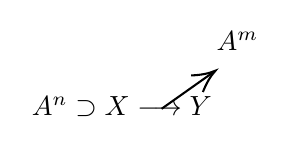
\begin{tikzpicture}[
                x=0.75pt,
                y=0.75pt,
                yscale=-1,
                xscale=1,
                every node/.style={text=black},
                every path/.style={draw=black},
                line width=0.75pt
            ]
                \draw    (340,140) -- (364.37,122.76) ;
                \draw [shift={(366,121.6)}, rotate = 144.71] [color={rgb, 255:red, 0; green, 0; blue, 0 }][line width=0.75]
                (10.93,-4.9) .. controls (6.95,-2.3) and (3.31,-0.67) .. (0,0) .. controls (3.31,0.67) and (6.95,2.3) .. (10.93,4.9);

                \draw (276,132.4) node [anchor=north west][inner sep=0.75pt] {$\mathbb{A}^{n} \supset X\longrightarrow Y$};
                \draw (365,101.4) node [anchor=north west][inner sep=0.75pt] {$\mathbb{A}^{m}$};
                \draw (359,119.4) node [anchor=north west][inner sep=0.75pt] {$\circlearrowright$};
            \end{tikzpicture}
        }
    \end{figure}

    Given $\vec{\pi} : \aa^n\to \aa^m$, we obtain a pullback homomorphism
    \[
        \pi^* : \kk[y_1,\ldots,y_m]\to \kk[x_1,\ldots,x_n].
    \]
    The condition that $\vec{\pi}(X)\subseteq Y$ is equivalent to saying that $\pi^*(I(Y))\subseteq I(X)$.
    Hence $\pi^*$ descends to a homomorphism
    \[
        \kk[Y] = \frac{\kk[y_1,\ldots,y_m]}{I(Y)} \to \frac{\kk[x_1,\ldots,x_n]}{I(X)} = \kk[X].
    \]

    Conversely, any $\kk$-algebra homomorphism $\kk[Y]\to \kk[X]$ determines a regular map $X\to Y$.
\end{proposition}

\begin{corollary}{
    There is a correspondence
    \[
        \{\text{affine varieties}\}\leftrightarrow\{\text{finitely generated reduced $\kk$-algebras}\}.
    \]
}
\end{corollary}

\begin{remark}
    For an abstract affine variety $X$, the choice of an embedding $X\hookrightarrow \aa^n$ is equivalent to the choice of algebra generators for $\kk[X]$.

    For example,
    \[
        \frac{\kk[x_1,x_2]}{(x_2 - x_1^2)} \cong \kk[y].
    \]
\end{remark}

\begin{lemma*}[More about Zariski Topology]{
    The following hold.
    \begin{enumerate}[label={(\arabic*)}]
    \item Closed subsets of an affine variety $X$ correspond to radical ideals in $\kk[X]$.
    \item The basic closed sets are $Z(f) = \{f = 0\}$, and the basic open sets are $D(f) = \{f\neq 0\}$.
    \item Regular maps are continuous.
    \item If $X$ is irreducible, then $\kk[X]$ has no zero divisors.
    \item $\kk[X]$ has no nilpotents.
    \item The Zariski topology is Noetherian.
    \item A homomorphism $\kk[Y]\to \kk[X]$ is surjective if and only if the corresponding map $X\to Y$ identifies $X$ with a closed subvariety of $Y$.
    \item A homomorphism $\kk[Y]\to \kk[X]$ is injective if and only if the image of the corresponding map $X\to Y$ is dense in $Y$.
    \end{enumerate}
}
\end{lemma*}

\begin{remark}[Elaboration on (1)]
    Suppose we have the topology $X$ on $\aa^n$ and a closed subset $Z\subseteq X$.

    \begin{figure}[H]
        \centering

        \tikzset{every picture/.style={line width=0.75pt}}

        \colorbox{white}{%
            \color{black}
            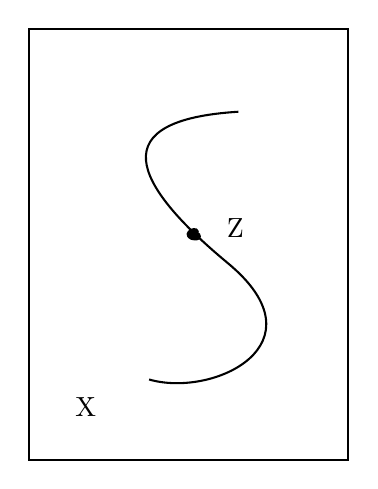
\begin{tikzpicture}[
                x=0.75pt,
                y=0.75pt,
                yscale=-1,
                xscale=1,
                every node/.style={text=black},
                every path/.style={draw=black},
                line width=0.75pt
            ]
                \draw   (253,22) -- (407,22) -- (407,229.78) -- (253,229.78) -- cycle ;
                \draw    (354,62) .. controls (289,66) and (302,96) .. (349,135) .. controls (396,174) and (342,200) .. (311,191) ;
                \draw  [line width=3] [line join = round][line cap = round] (333,120) .. controls (331.45,120) and (328.95,122) .. (334,122) ;

                \draw (347,112) node [anchor=north west][inner sep=0.75pt] {Z};
                \draw (274,198) node [anchor=north west][inner sep=0.75pt] {X};
            \end{tikzpicture}
        }
    \end{figure}

    Note that $Z\subseteq X\subseteq \aa^n$.
    Then we have
    \[
        I(Z)\supseteq I(X).
    \]
\end{remark}

\begin{definition}[Topology on a Set]
    A topology on a set $S$ consists of closed sets $Z_\alpha$ and open sets $U_\alpha$.
    In the Zariski topology, the basic closed sets are
    \[
        Z(f) = \{f = 0\},
    \]
    and the basic open sets are
    \[
        D(f) = \{f\neq 0\}.
    \]
\end{definition}

\begin{remark}[Elaboration on (3)]
    Recall that for a regular map $\pi : X\to Y$, and for a closed set $Z(f)\subseteq Y$, we have
    \[
        \pi^{-1}(Z(f)) = Z(\pi^*(f)).
    \]

    \begin{figure}[H]
        \centering

        \tikzset{every picture/.style={line width=0.75pt}}

        \colorbox{white}{%
            \color{black}
            \begin{tikzpicture}[
                x=0.75pt,
                y=0.75pt,
                yscale=-1,
                xscale=1,
                every node/.style={text=black},
                every path/.style={draw=black},
                line width=0.75pt
            ]
                \draw (216,73.4) node [anchor=north west][inner sep=0.75pt] {$\mathbb{A}^{n}$};
                \draw (215,100.4) node [anchor=north west][inner sep=0.75pt] {$\uparrow$};
                \draw (219,126.4) node [anchor=north west][inner sep=0.75pt] {$X\underset{\pi}{\rightarrow} Y$};
                \draw (252,74.4) node [anchor=north west][inner sep=0.75pt] {$\mathbb{A}^{m}$};
                \draw (251,101.4) node [anchor=north west][inner sep=0.75pt] {$\uparrow$};
                \draw (251,148.4) node [anchor=north west][inner sep=0.75pt] {$\cup$};
                \draw (245,169.4) node [anchor=north west][inner sep=0.75pt] {$Z(f)$};
                \draw (229,105.4) node [anchor=north west][inner sep=0.75pt] {$\nearrow$};
                \draw (303,99.4) node [anchor=north west][inner sep=0.75pt] {$ \begin{array}{l}
                                                                                   \mathbb{K}[X]\leftarrow \mathbb{K}[Y]\\
                                                                                   \pi^*(f)\mapsfrom f
                \end{array}$};
            \end{tikzpicture}
        }
    \end{figure}
\end{remark}

\begin{definition}[Irreducible]
    A variety $X$ is irreducible if it cannot be written as
    \[
        X = Z_1\cup Z_2
    \]
    with $Z_1,Z_2\subsetneq X$ both closed.
\end{definition}

\begin{remark}[Elaboration on (4)]
    In an ordinary topology on $\rr$, one often studies decompositions into unions of subsets.
    Here, for irreducibility, it is enough to consider closed subsets.

    If
    \[
        Z(f_1)\cup Z(f_2) = X,
    \]
    then irreducibility says that one of these must already equal $X$.
\end{remark}

\begin{definition}[Connected]
    A space is connected if it cannot be written as a disjoint union of two nonempty subsets that are both open and closed.
\end{definition}

\begin{definition}[Idempotence]
    An element $e\in R$ is idempotent if
    \[
        e^2 = e.
    \]
\end{definition}

\begin{lemma*}{
    If
    \[
        X = Z_1\cup\cdots\cup Z_k
    \]
    is a finite union of irreducible closed subsets, and no $Z_i$ is contained in another $Z_j$, then the $Z_i$ are the irreducible components of $X$.
}
\end{lemma*}

\begin{definition}[Closure]
    The closure of a subset is the intersection of all closed sets containing it.
\end{definition}

Now assume that $X$ is an irreducible affine variety.
Then $R = \kk[X]$ has no zero divisors.
We already have the quotient field
\[
    \kk(X) = \Frac(R),
\]
where $\varphi\in \kk(X)$ is a rational function
\[
    \varphi : U\to \kk
\]
defined on some nonempty open subset $U\subseteq X$.

\begin{figure}[H]
    \centering

    \tikzset{every picture/.style={line width=0.75pt}}

    \colorbox{white}{%
        \color{black}
        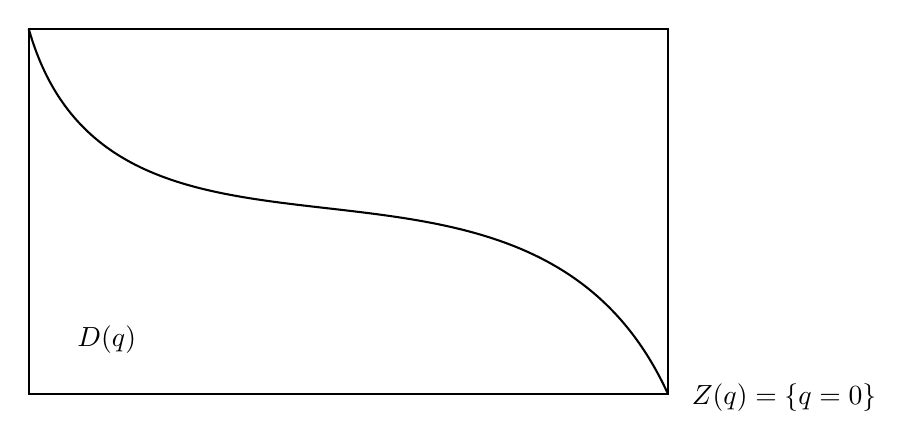
\begin{tikzpicture}[
            x=0.75pt,
            y=0.75pt,
            yscale=-1,
            xscale=1,
            every node/.style={text=black},
            every path/.style={draw=black},
            line width=0.75pt
        ]
            \draw   (165,41) -- (473,41) -- (473,217) -- (165,217) -- cycle ;
            \draw    (165,41) .. controls (206,186) and (405,68) .. (473,217) ;

            \draw (483,210.4) node [anchor=north west][inner sep=0.75pt] {$Z(q) = \{q = 0\}$};
            \draw (187,182.4) node [anchor=north west][inner sep=0.75pt] {$D(q)$};
        \end{tikzpicture}
    }
\end{figure}

\begin{lemma}{
    If $X$ is irreducible and $U_1,U_2\subseteq X$ are nonempty open subsets, then
    \[
        U_1\cap U_2\neq \varnothing.
    \]
}
    If $U_1\cap U_2 = \varnothing$, then
    \[
        X = (X\setminus U_1)\cup (X\setminus U_2),
    \]
    where both complements are proper closed subsets of $X$.
    This contradicts irreducibility.
\end{lemma}